\chapter{Conclusion}
\label{chap:conclusion}
	Pressure ulcers and deep tissue injuries are an incredible problem facing the health of society today. They arise most often as complications in the elderly and those with spinal cord injuries and present an extremely significant burden on both the health care system and individual patients alike. Deep tissue injuries are somewhat more insidious than pressure ulcers due to how they form---deep tissue injuries begin at the bone-muscle interface deep within tissue and aren't readily noticeable on the surface of the skin until they have broken through as late-stage pressure ulcers. Although DTI prevention and mitigation strategies do exist, their efficacy is highly variable and the treatments are largely untargeted blanket programs which may not adequately treat the needs of patients with formative DTI and may waste money on those without issue. Without a proper clinical diagnostic capability, the incidence of pressure ulcers and DTI has remained largely unchanged for decades. Currently, the only tool capable of detecting formative deep tissue injuries in their early stages---before they tunnel to the surface---is $\mathrm{T}_2^*$-weighted MRI which images oxygen content (or lack thereof) as a proxy for tissue health. While MRI may be effective in research settings, it is hardly suitable for large-scale clinical adoption due to the excessive monetary and temporal costs as well as it's lack of mobility and lack of ability to image people with critical medical implants such as pacemakers.

	Ultrasound elastography is a relatively new imaging modality that has shown some promise toward the detection of early deep tissue injuries by imaging the stiffness changes that tissue undergoes beginning immediately after an injury has occurred---injured tissue shows 1.6-fold to 3.3-fold stiffening after the initial injury and after becoming necrotic shows stiffness below that of healthy tissue. There are three main technologies relating to ultrasound elastography: quasi-static elastography, acoustic radiation force impulse imaging, and shear wave speed quantification. Quasi-static ultrasound elastography is a technique whereby the deflection and deformation of acoustic scatterers embedded throughout soft tissue are tracked between externally-applied pre- and post- compression states. Regions of tissue which deform less than their surroundings are mechanically stiffer than their surroundings and may represent a formative deep tissue injury. Acoustic radiation force impulse imaging operates on much the same principle as this, however the externally-induced tissue deformation is generated through the application of acoustic radiation forces stemming from specialized pulses emitted from the ultrasound transducer itself. By generating tissue deformation in this manner, the repeatability and inter-operator reliability of diagnostic scans may be improved due to the automatic and computer-controlled nature of the acoustic radiation forces. While quasi-static ultrasound elastography and acoustic radiation force impulse imaging provide only qualitative measures of tissue stiffness relative to it's surroundings, shear-wave speed quantification can provide quantitative measures of tissue elasticity through the direct computation of a region of tissue's shear modulus by it's measured velocity and an assumed tissue density. Shear-wave speed quantification tracks the velocity of shear waves generated using an acoustic radiation force as they pass through both diseased and healthy tissue using regular ultrasound tracking beams sampled at extremely high frequencies. Through these methods, it is expected that a clinical tool may be developed for not only detecting the early onset of deep tissue injuries but also for tracking their progress over time. The work completed here represents the first step in that goal and numerically characterized the use of all three techniques toward the detection of both early and late-stage deep tissue injuries.

	\section{Comparisons Between Methods}
	\label{sec:method_comparisons}
		In the quest to understand the use of the various ultrasound elastography imaging modalities toward early detection of deep tissue injuries, the sensitivity of numerous parameters relating to each modality were studied. Amongst the studied parameters, a subset of studies are directly comparable between modalities---parameters such as lesion size, depth, blur radius, cluster density, and the use of ``real-world'' geometry were all examined at parametrically identical values. This allows the direct comparison between modalities and may lead to recommendations for future clinical use of ultrasound elastography.

		\subsubsection{Simulated Lesions}
		\label{subsubsec:conclusion_simulated_lesions}
			Across the range of simulated lesions using the quasi-static elastography, ARFI imaging, and shear wave speed quantification modalities, hard boundaried lesions represent the most ``basic'' and general case used to investigate overarching lesion parameters such as overall size of the lesion and the depth at which it is placed. In order to compare the investigated modalities, a cross-section of the data centred around a lesion with radius of \SI{10}{\mm} at a depth of \SI{4}{\cm} is shown in Fig. \ref{fig:conclusion_radius}. In Fig. \ref{fig:conclusion_radius}, it is clear to see that shear wave speed quantification is by far the most accurate of the three detection modalities with its characterization curve representing an almost ideal one-to-one mapping of measured stiffness to true stiffness. Quasi-static elastography and ARFI imaging resulted in less detection sensitivity and were not substantially different from each other.

			\begin{figure}[!htb]
				\centering
				\begin{tikzpicture}
					\begin{axis}[
						scale only axis,
						height=2.5in,
						width=\textwidth-\widthof{100}-1in,
						xlabel={Nominal Stiffness Ratio, $E_{nom}$},
						ylabel={Measured Stiffness Ratio, $E_{rel,measured}$},
						grid=major,
						legend entries={Quasi-Static, ARFI, Shear, Ideal},
						legend style={legend pos=north west,font=\small},
						clip=true,
						cycle list name=ColourPlotCycle,
						draw=black, text=black, fill=black,
						xmin=0, xmax=3.5,
						ymin=0, ymax=3.5]
						\addplot table {assets/quasistatic/data/circular_size_20.dat};
						\addplot table {assets/arfi/data/arfi_radius_r100.dat};
						\addplot table {assets/shear/data/shear_radius_r100.dat};
						\addplot[mark=none,dashed,ultra thick] plot coordinates {(0, 0) (4, 4)};
						\node (c) at (axis cs:3,0.75) {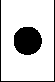
\includegraphics{assets/quasistatic/insets/inset_single.pdf}};
					\end{axis}
				\end{tikzpicture}
				\caption[Detection sensitivities of hard-boundaried spherical lesions using the three investigated imaging modalities]{Detection sensitivities of hard-boundaried spherical lesions with radii of \SI{10}{\mm} at a depth of \SI{4}{\cm} using quasi-static elastography, ARFI imaging, and shear wave speed quantification.}
				\label{fig:conclusion_radius}
			\end{figure}

			To further examine the error introduced by the various detection modalities, the percent difference between the expected true values of lesion stiffness and the measured lesion stiffness for the results seen in Fig. \ref{fig:conclusion_radius} are shown in Fig. \ref{fig:conclusions_radius_pd}. Fig. \ref{fig:conclusions_radius_pd} shows that in across all lesion stiffnesses, shear wave speed quantification results in the least amount of error between the true and measured lesion stiffness. Errors across all the modalities were greatest for the softest lesions---those with stiffness ratios of 0.32. Errors involved with ARFI imaging were slightly greater than for quasi-static imaging across the remaining investigated stiffness ratios. It is likely however that the slight increase in error associated with ARFI imaging may be worth the added benefit of increased reliability and repeatability. Beyond this, shear wave speed quantification is certainly recommended for detecting lesions if at all possible not only due to its nature of fully quantifying tissue stiffness rather than simply estimating it but also due to it's superior accuracy over quasi-static elastography and ARFI imaging.

			\begin{figure}[!htb]
				\centering
				\begin{tikzpicture}
					\begin{axis}[
						scale only axis,
						height=2.5in,
						width=\textwidth-\widthof{100}-1in,
						major x tick style = transparent,
						ybar=2*\pgflinewidth,
						legend entries={Quasi-Static, ARFI, Shear},
						legend style={legend pos=north east,font=\small},
						bar width=14pt,
						ymajorgrids=true,
						xlabel={Nominal Stiffness Ratio, $E_{nom}$},
						ylabel={Percent Error (\si{\percent})},
						enlarge x limits=0.25,
						symbolic x coords={0.32, 0.56, 1.8, 3.2},
						xticklabels={0.32, 0.56, 1.80, 3.20},
						xtick=data,
						ymin=0,
						cycle list name=BarColourPlotCycle]
						\pgfplotstableread{assets/conclusions/conclusion_radius.dat}{\conclusionRadius}
						\addplot table[x={trueSR}, y={quasiPD}] {\conclusionRadius};
						\addplot table[x={trueSR}, y={arfiPD}] {\conclusionRadius};
						\addplot table[x={trueSR}, y={shearPD}] {\conclusionRadius};
					\end{axis}
				\end{tikzpicture}
				\caption[Percent error of measured stiffness ratios for spherical lesions across the three investigated modalities]{Percent error of measured stiffness ratios for spherical lesions with radii of \SI{10}{\mm} at a depth of \SI{4}{\cm} across the three investigated modalities.}
				\label{fig:conclusions_radius_pd}
			\end{figure}

			Since it is highly unlikely that real-world lesions will present as perfectly spherical, hard-boundaried lesions, different lesion geometries were studied. One such case is where a lesion will not have rigidly defined boundaries and may ``fade'' into the background healthy tissue. To investigate this, lesions with blurred boundaries that fade into the background were studied using all three elastography modalities. The characterization curves of a lesion with a radius of \SI{10}{\mm} which was blurred using a kernel blur radius of \SI{7.5}{\mm} across the three modalities are given in Fig. \ref{fig:conclusion_blur}. As expected, shear wave speed quantification again revealed itself to produce the most accurate results with a nearly one-to-one mapping between true and measured lesion stiffness. Quasi-static elastography and ARFI imaging paralleled each other however quasi-static elastography was generally unable to distinguish soft blurred lesions against the background, making ARFI imaging much more preferable than quasi-static elastography when examining late-stage DTI.

			\pgfplotstableread{assets/conclusions/conclusion_blur.dat}{\conclusionBlur}
			\begin{figure}[!htb]
				\centering
				\begin{tikzpicture}
					\begin{axis}[
						scale only axis,
						height=2.5in,
						width=\textwidth-\widthof{100}-1in,
						xlabel={Nominal Stiffness Ratio, $E_{nom}$},
						ylabel={Measured Stiffness Ratio, $E_{rel,measured}$},
						grid=major,
						legend entries={Quasi-Static, ARFI, Shear, Ideal},
						legend style={legend pos=north west,font=\small},
						clip=true,
						cycle list name=ColourPlotCycle,
						draw=black, text=black, fill=black,
						xmin=0, xmax=3.5,
						ymin=0, ymax=3.5]
						\addplot table[x={trueSR}, y={quasiSR}] {\conclusionBlur};
						\addplot table[x={trueSR}, y={arfiSR}] {\conclusionBlur};
						\addplot table[x={trueSR}, y={shearSR}] {\conclusionBlur};
						\addplot[mark=none,dashed,ultra thick] plot coordinates {(0, 0) (4, 4)};
						\node (c) at (axis cs:3,0.75) {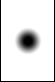
\includegraphics{assets/quasistatic/insets/inset_blur.pdf}};
					\end{axis}
				\end{tikzpicture}
				\caption[Detection sensitivities of blurred-boundary spherical lesions using the three investigated imaging modalities]{Detection sensitivities of blurred-boundary spherical lesions with radii of \SI{10}{\mm} with blur radii of \SI{7.5}{\mm} using quasi-static elastography, ARFI imaging, and shear wave speed quantification.}
				\label{fig:conclusion_blur}
			\end{figure}

			Again as expected, shear wave speed quantification resulted in substantially less error for characterizing all stages of deep tissue injuries than both quasi-static elastography and ARFI imaging as Fig. \ref{fig:conclusions_blur_pd} shows. Once again, the softest lesions that were investigated---those with a relative stiffness ratio of 0.32---were the most difficult to detect accurately and presented with the greatest amount of error. Of further note is that although quasi-static elastography was worse at accurately detecting soft deep tissue injury lesions than ARFI imaging, quasi-static elastography portrayed less error when detecting stiff (early) deep tissue injury lesions. This suggests that quasi-static elastography is not well suited for detecting soft lesions and that the more reliable ARFI imaging should be used where possible if shear wave speed quantification cannot be used.

			\begin{figure}[!htb]
				\centering
				\begin{tikzpicture}
					\begin{axis}[
						scale only axis,
						height=2.5in,
						width=\textwidth-\widthof{100}-1in,
						major x tick style = transparent,
						ybar=2*\pgflinewidth,
						legend entries={Quasi-Static, ARFI, Shear},
						legend style={legend pos=north east,font=\small},
						bar width=14pt,
						ymajorgrids=true,
						xlabel={Nominal Stiffness Ratio, $E_{nom}$},
						ylabel={Percent Error (\si{\percent})},
						enlarge x limits=0.25,
						symbolic x coords={0.32, 0.56, 1.8, 3.2},
						xticklabels={0.32, 0.56, 1.80, 3.20},
						xtick=data,
						cycle list name=BarColourPlotCycle]
						\addplot table[x={trueSR}, y={quasiPD}] {\conclusionBlur};
						\addplot table[x={trueSR}, y={arfiPD}] {\conclusionBlur};
						\addplot table[x={trueSR}, y={shearPD}] {\conclusionBlur};
					\end{axis}
				\end{tikzpicture}
				\caption[Percent error of measured stiffness ratios for blurred lesions across the three investigated modalities]{Percent error of measured stiffness ratios for blurred lesions with radii of \SI{10}{\mm} and blur radii of \SI{7.5}{\mm} across the three investigated modalities.}
				\label{fig:conclusions_blur_pd}
			\end{figure}

			Since lesionous regions may not be completely homogeneous regions of injured tissue, a model comprising numerous small lesions clustered together to form a greater lesionous region was developed. Fig. \ref{fig:conclusion_cluster} shows a cross-section of the characterization curves for this model when small lesions with radii of \SI{1}{\mm} were clustered with a density of \SI{20}{\per\cm\squared}. Although none of the investigated modalities were able to distinguish individual lesions in the various cluster models, all were able to differentiate the lesionous region as a whole. Once again, shear wave speed quantification proved to be the most accurate method with it's characterization curves coming the closest to a one-to-one mapping of true to measured stiffnesses. Of note in this case, however, is that even shear wave speed quantification was still substantially less sensitive to lesions than an ideal case---all investigated modalities both over-estimated the stiffness of soft lesions and under-estimated the stiffness of stiff lesions.

			\pgfplotstableread{assets/conclusions/conclusion_cluster.dat}{\conclusionCluster}
			\begin{figure}[!htb]
				\centering
				\begin{tikzpicture}
					\begin{axis}[
						scale only axis,
						height=2.5in,
						width=\textwidth-\widthof{100}-1in,
						xlabel={Nominal Stiffness Ratio, $E_{nom}$},
						ylabel={Measured Stiffness Ratio, $E_{rel,measured}$},
						grid=major,
						legend entries={Quasi-Static, ARFI, Shear, Ideal},
						legend style={legend pos=north west,font=\small},
						clip=true,
						cycle list name=ColourPlotCycle,
						draw=black, text=black, fill=black,
						xmin=0, xmax=3.5,
						ymin=0, ymax=3.5]
						\addplot table[x={trueSR}, y={quasiSR}] {\conclusionCluster};
						\addplot table[x={trueSR}, y={arfiSR}] {\conclusionCluster};
						\addplot table[x={trueSR}, y={shearSR}] {\conclusionCluster};
						\addplot[mark=none,dashed,ultra thick] plot coordinates {(0, 0) (4, 4)};
						\node (c) at (axis cs:3,0.75) {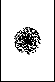
\includegraphics{assets/quasistatic/insets/inset_blob.pdf}};
					\end{axis}
				\end{tikzpicture}
				\caption[Detection sensitivities of clustered lesions using the three investigated imaging modalities]{Detection sensitivities of clustered lesions with a cluster density of \SI{20}{\per\cm\squared} and individual radii of \SI{1}{\mm} using quasi-static elastography, ARFI imaging, and shear wave speed quantification.}
				\label{fig:conclusion_cluster}
			\end{figure}

			The lesser detection sensitivity with all investigated imaging modalities that was portrayed in Fig. \ref{fig:conclusion_cluster} results in a greater amount of error across all imaging modalities and lesion stiffness ratios as seen in Fig. \ref{fig:conclusions_cluster_pd}. For all but the softest of lesions, ARFI imaging had the greatest amount of error when attempting to detect these lesionous clusters, while shear wave speed quantification continued to generally produce the least amount of error. The overall increased error in this model is somewhat expected however, due to the nature of how the models were constructed and evaluated. In the clustered lesion models, only a portion of the lesionous region actually contains ``injured'' tissue---averaging out the true stiffness over the entire lesionous area would result in a less pronounced stiffness for that region, rather than the ``spikes'' that are seen in the clustered model. This means that if such a lesionous region were to exist, the severity of the injury may not be adequately represented by \emph{any} of the three imaging modalities. Further work should be done to examine this problem further and investigate any alternative technologies which may be able to adequately granularize clusters of small lesions.

			\begin{figure}[!htb]
				\centering
				\begin{tikzpicture}
					\begin{axis}[
						scale only axis,
						height=2.5in,
						width=\textwidth-\widthof{100}-1in,
						major x tick style = transparent,
						ybar=2*\pgflinewidth,
						legend entries={Quasi-Static, ARFI, Shear},
						legend style={legend pos=north east,font=\small},
						bar width=14pt,
						ymajorgrids=true,
						xlabel={Nominal Stiffness Ratio, $E_{nom}$},
						ylabel={Percent Error (\si{\percent})},
						enlarge x limits=0.25,
						symbolic x coords={0.32, 0.56, 1.8, 3.2},
						xticklabels={0.32, 0.56, 1.80, 3.20},
						xtick=data,
						cycle list name=BarColourPlotCycle]
						\addplot table[x={trueSR}, y={quasiPD}] {\conclusionCluster};
						\addplot table[x={trueSR}, y={arfiPD}] {\conclusionCluster};
						\addplot table[x={trueSR}, y={shearPD}] {\conclusionCluster};
					\end{axis}
				\end{tikzpicture}
				\caption[Percent error of measured stiffness ratios for clustered lesions across the three investigated modalities]{Percent error of measured stiffness ratios for clustered lesions with a cluster density of \SI{20}{\per\cm\squared} and individual radii of \SI{1}{\mm} across the three investigated modalities.}
				\label{fig:conclusions_cluster_pd}
			\end{figure}

			The final major model to be evaluated across quasi-static elastography, ARFI imaging, and shear wave speed quantification was the use of geometry obtained from MRI scans of real deep tissue injuries in pigs which were then placed in a background of tissue with geometry obtained from the Visible Human project. The purpose of these models was to place the various simulation techniques in the context of detecting ``real-world'' deep tissue injury lesions. The characterization curves of the three investigated modalities for a lesion with a width of \SI{20}{\mm} located at a depth of \SI{6}{\cm} are given in Fig. \ref{fig:conclusion_human}. A lesion depth of \SI{6}{\cm} was chosen in these models as in the Visible Human tissue domain this depth placed the lesion to sit immediately superior to the ischial tuberosity---a boney prominence often associated with deep tissue injuries. As Fig. \ref{fig:conclusion_human} shows, shear wave speed quantification once again presented the most ideal detection sensitivity of the three modalities. Both quasi-static elastography and ARFI imaging were much less sensitive to lesions in this model, with soft lesions being almost impossible to detect using quasi-static elastography. A key differentiation in this Visible Human model from the hard-boundaried spherical model studied previously is that shear wave speed quantification grossly underestimated the stiffness of both the softest and stiffest lesions examined.

			\pgfplotstableread{assets/conclusions/conclusion_human.dat}{\conclusionHuman}
			\begin{figure}[!htb]
				\centering
				\begin{tikzpicture}
					\begin{axis}[
						scale only axis,
						height=2.5in,
						width=\textwidth-\widthof{100}-1in,
						xlabel={Nominal Stiffness Ratio, $E_{nom}$},
						ylabel={Measured Stiffness Ratio, $E_{rel,measured}$},
						grid=major,
						legend entries={Quasi-Static, ARFI, Shear, Ideal},
						legend style={legend pos=north west,font=\small},
						clip=true,
						cycle list name=ColourPlotCycle,
						draw=black, text=black, fill=black,
						xmin=0, xmax=3.5,
						ymin=0, ymax=3.5]
						\addplot table[x={trueSR}, y={quasiSR}] {\conclusionHuman};
						\addplot table[x={trueSR}, y={arfiSR}] {\conclusionHuman};
						\addplot table[x={trueSR}, y={shearSR}] {\conclusionHuman};
						\addplot[mark=none,dashed,ultra thick] plot coordinates {(0, 0) (4, 4)};
						\node (c) at (axis cs:1.5,2.75) {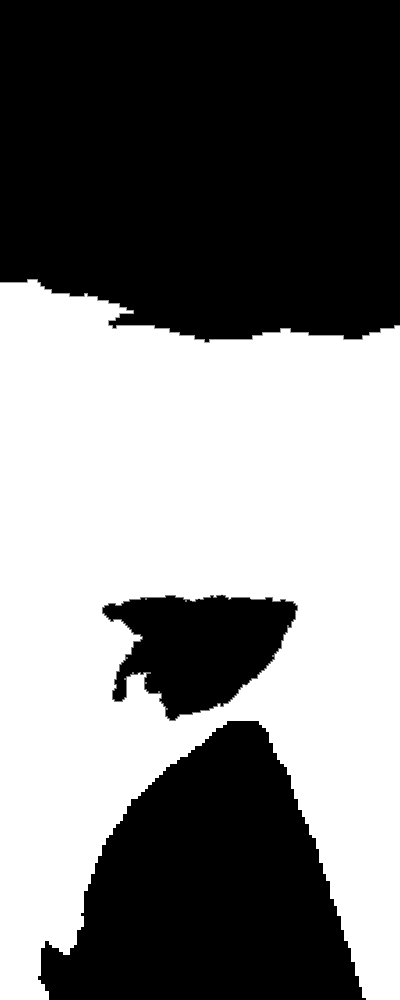
\includegraphics[width=0.072\columnwidth]{assets/quasistatic/insets/human.png}};
						\node (rect) at (axis cs:1.5,2.75) [draw,minimum width=0.072\columnwidth,minimum height=0.18\columnwidth]{};
					\end{axis}
				\end{tikzpicture}
				\caption[Detection sensitivities of MRI-acquired Visible Human lesions using the three investigated imaging modalities]{Detection sensitivities of MRI-acquired Visible Human lesions with a width of \SI{20}{\mm} at a depth of \SI{6}{\cm} using quasi-static elastography, ARFI imaging, and shear wave speed quantification.}
				\label{fig:conclusion_human}
			\end{figure}

			As Fig. \ref{fig:conclusions_human_pd} shows, the error for shear wave speed quantification is much greater for both very soft ($E_{nom} = 0.32$) and very stiff ($E_{nom} = 3.20$) lesions---the error for soft lesions even surpasses that of ARFI imaging for the first time. For all other nominal stiffness ratios, shear wave speed quantification once again outperformed both quasi-static elastography and ARFI imaging. Although the use of more complicated geometry in the Visible Human project decreased the accuracy of shear wave speed quantification, it was once again the most sensitive and accurate of the investigated imaging modalities, suggesting it be used for quantifying deep tissue injuries if at all possible.

			\begin{figure}[!htb]
				\centering
				\begin{tikzpicture}
					\begin{axis}[
						scale only axis,
						height=2.5in,
						width=\textwidth-\widthof{100}-1in,
						major x tick style = transparent,
						ybar=2*\pgflinewidth,
						legend entries={Quasi-Static, ARFI, Shear},
						legend style={legend pos=north east,font=\small},
						bar width=14pt,
						ymajorgrids=true,
						xlabel={Nominal Stiffness Ratio, $E_{nom}$},
						ylabel={Percent Error (\si{\percent})},
						enlarge x limits=0.25,
						symbolic x coords={0.32, 0.56, 1.8, 3.2},
						xticklabels={0.32, 0.56, 1.80, 3.20},
						xtick=data,
						cycle list name=BarColourPlotCycle]
						\addplot table[x={trueSR}, y={quasiPD}] {\conclusionHuman};
						\addplot table[x={trueSR}, y={arfiPD}] {\conclusionHuman};
						\addplot table[x={trueSR}, y={shearPD}] {\conclusionHuman};
					\end{axis}
				\end{tikzpicture}
				\caption[Percent error of measured stiffness ratios for MRI-acquired Visible Human lesions across the three investigated modalities]{Percent error of measured stiffness ratios for MRI-acquired Visible Human lesions with a width of \SI{20}{\mm} at a depth of \SI{6}{\cm} across the three investigated modalities.}
				\label{fig:conclusions_human_pd}
			\end{figure}

		\FloatBarrier
		\subsubsection{Experimental Validations}
			In the experiments that were performed with each of the three elastography modalities on a tissue mimicking phantom, all three methodologies were able to distinguish both hard and soft lesions with some degree of accuracy. However, the stiffest lesions that were examined---those with a nominal stiffness ratio of 3.2---presented the greatest error and variation in the results as seen in Fig. \ref{fig:compare_nominal_experiments}. In these experiments, both ARFI imaging and shear wave speed quantification score similarly, although the variation in the shear results was much greater than the variation in the ARFI experiments. Both ARFI imaging and shear wave speed quantification showed relatively similar detection sensitivities with the major difference between the two being that ARFI imaging consistently over-estimated lesion stiffness as compared to shear wave speed quantification. Shear wave speed quantification was found to be the most accurate for ``soft'' lesions, while ARFI imaging performed marginally better with stiff lesions. Quasi-static elastography generally displayed the worst results, echoing what was seen in Section \ref{subsubsec:conclusion_simulated_lesions}.

			\begin{figure}[!htb]
				\centering
				\begin{tikzpicture}
					\begin{axis}[
						scale only axis,
						height=2.5in,
						width=\textwidth-\widthof{100}-1in,
						xlabel={Nominal Stiffness Ratio, $E_{nominal}$},
						ylabel style={align=center},
						ylabel={Experimentally Measured \\ Stiffness Ratio, $E_{exp,measured}$},
						legend entries={Quasi-Static, ARFI, Shear, Ideal},
						legend style={legend pos=north west,font=\small},grid=major,clip=true,cycle list name=ColourPlotCycle,
						xmin=0, xmax=4,
						ymin=0, ymax=4,
						draw=black, text=black, fill=black]
							\addplot table {assets/quasistatic/data/validation_nominal.dat};
							\addplot+[
								error bars/.cd,
								y dir=both,
								y explicit,
								error bar style={ultra thick},
								error mark options={
									rotate=90,
									mark size=8pt,
									ultra thick
								}] table[y error plus=upper, y error minus=lower] {assets/arfi/data/arfi_experiment_nominal.dat};
							\addplot+[
								error bars/.cd,
								y dir=both,
								y explicit,
								error bar style={ultra thick},
								error mark options={
									rotate=90,
									mark size=8pt,
									ultra thick
								}] table[y error plus=upper, y error minus=lower] {assets/shear/data/shear_experiment_nominal.dat};
							\addplot[mark=none,dashed,ultra thick] plot coordinates {(0, 0) (4, 4)};
						\node (c) at (axis cs:3.5,0.75) {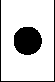
\includegraphics{assets/quasistatic/insets/inset_single.pdf}};
					\end{axis}
				\end{tikzpicture}
				\caption[Experimental results of the three methodologies investigated]{Experimental results of the three methodologies investigated. ARFI imaging consistently overestimated the stiffness of the lesion compared to both quasi-static and shear wave speed quantification, which generally underestimated the stiffness of lesions.}
				\label{fig:compare_nominal_experiments}
			\end{figure}

			By comparing the simulated results presented throughout this work to the parametrically identical results obtained through experiment, the accuracy of the simulations apart from the overall accuracy of the technique may be determined. These results are compared in Fig. \ref{fig:compare_experiments} which shows a general agreement between experimentally measured stiffness ratios and their simulated counterparts for all but stiff ARFI imaging-acquired lesions. Since the simulation results for quasi-static elastography and shear wave speed quantification fall within error of their experimental counterparts, these simulation paradigms may be deemed acceptable. Counter to this, the simulation-acquired stiffness ratios in ARFI imaging fall well below their experimental values, suggesting that the current ARFI imaging simulation methodology is insufficient in accurately reproducing real-world results and that future work is necessary to more closely align the ARFI imaging models with reality.

			\begin{figure}[!htb]
				\centering
				\begin{tikzpicture}
					\begin{axis}[
						scale only axis,
						height=2.5in,
						width=\textwidth-\widthof{100}-1in,
						xlabel={Experimentally Measured Stiffness Ratio, $E_{exp,measured}$},
						ylabel style={align=center},
						ylabel={Simulated Measured \\ Stiffness Ratio, $E_{sim,measured}$},
						legend entries={Quasi-Static, ARFI, Shear, Ideal},
						legend style={legend pos=north west,font=\small},grid=major,clip=true,cycle list name=ColourPlotCycle,
						xmin=0, xmax=4,
						ymin=0, ymax=4,
						draw=black, text=black, fill=black]
							\addplot table {assets/quasistatic/data/validation.dat};
							\addplot+[
								error bars/.cd,
								x dir=both,
								x explicit,
								error bar style={ultra thick},
								error mark options={
									rotate=90,
									mark size=8pt,
									ultra thick
								}] table[x error plus=upper, x error minus=lower] {assets/arfi/data/arfi_experiment.dat};
							\addplot+[
								error bars/.cd,
								x dir=both,
								x explicit,
								error bar style={ultra thick},
								error mark options={
									rotate=90,
									mark size=8pt,
									ultra thick
								}] table[x error plus=upper, x error minus=lower] {assets/shear/data/shear_experiment.dat};
							\addplot[mark=none,dashed,ultra thick] plot coordinates {(0, 0) (4, 4)};
						\node (c) at (axis cs:3.5,0.75) {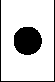
\includegraphics{assets/quasistatic/insets/inset_single.pdf}};
					\end{axis}
				\end{tikzpicture}
				\caption[Experimental validation of the simulation results across all three methodologies investigated]{Experimental validation of the simulation results across all three methodologies investigated. The quasi-static ultrasound elastography and shear wave speed quantification simulations most closely matched the results seen experimentally.}
				\label{fig:compare_experiments}
			\end{figure}

	\section{Recommendations and Future Work}
		The work presented in Chapters \ref{chap:quasi-static} -- \ref{chap:shear} represents a numerical characterization of three different ultrasound elastography imaging modalities: quasi-static ultrasound elastography, acoustic radiation force impulse imaging, and shear wave speed quantification. From the results presented in these chapters the critical parameters relating to detecting both formative and progressive deep tissue injuries across all three detection modalities were investigated. These parameters included device-design specifics such as: frequency; transmit pressure; transducer size; etc, as well as physical lesion-specific parameters such as: depth; size; geometry; etc. Through the comparisons made in Section \ref{sec:method_comparisons}, it is clear that shear wave speed quantification is the ideal ultrasound elastography modality with regards to detecting deep tissue injuries. Not only is shear wave speed quantification a quantifiable technology which would allow clinicians to directly track the progression of an injury over time, but it was found to consistently provide the most accurate results compared to both quasi-static elastography and ARFI imaging. Shear wave speed quantification is not without its limits however, as the acoustic radiation force impulses which give rise to deformation deep within tissue may not be large enough to be readily detected by the ultrasound machine. To overcome these limitations, the ultrasonic transmission power may be increased and the interrogation frequency may be decreased, but such measures may only go so far and have profound tissue health implications. Further, since a specific region of tissue must be interrogated using shear wave speed quantification, quasi-static ultrasound elastography or ARFI imaging may be used to image much larger regions of tissue in order to search for specific regions of interest. Although such ``fishing'' expeditions may not stand well on their own, they may guide the use of shear wave speed quantification to provide a more complete picture of tissue health.

		From the work presented here, it is fully expected that ultrasound elastography is capable of becoming a clinical tool to be used in the early detection and monitoring of deep tissue injuries. The adoption of this technology for such a venture would have wide-ranging consequences from potentially increasing quality of life of at-risk patients, to decreasing the financial burden on the health care system, to even providing future avenues for deep tissue injury research---without a quality early deep tissue injury detection method, the bulk of deep tissue injury research focuses on late-stage ulcers for which treatments are often applied ``too late''. With a firm understanding of the mechanics and principles involved with ultrasound elastography, the next stage in this technology's development is to investigate its use in animal models where deep tissue injury lesions may be tightly controlled and the lesions can be co-investigated using MRI techniques. Once early deep tissue injury detection is well understood in living tissue, trials should move to at-risk human patients. Since ultrasound and subsequently ultrasound elastography are non-invasive tools with relatively inexpensive equipment, it is expected that clinical adoption will be swift once the technology is proven in human tissue. Although as of the time of writing there are commercially available ultrasound elastography systems, future work may involve developing application-specific probes or even entire devices devoted to applying ultrasound elastography toward deep tissue injuries which can provide the necessary parameters to optimize detection and ease of use.

		Ultrasound elastography is a powerful tool which through the numerical simulations performed in this work was found to be able to distinguish both early and late stage deep tissue injuries and may provide for the first ever clinical tool to reliably detect DTI with a thought toward improving patient care and quality of life.

\bibcomplete{references}